\documentclass[12pt]{article}

% packages
\usepackage{setspace}
\usepackage{array}
\usepackage[margin=0.75in]{geometry}
\usepackage{amsmath,bm}
\usepackage{amssymb}
\usepackage{bbold}
\usepackage{physics}
\usepackage{xcolor}
\usepackage{indentfirst}
\usepackage{enumerate}
\usepackage{mathtools}
\usepackage{fancyhdr}
\usepackage{hyperref}


\pagestyle{fancy}
\fancyhf{}
\rhead{Creative Destruction Lab}
\lhead{Introductions to Projects}
\rfoot{Page \thepage}

\allowdisplaybreaks

\title{CDL Quantum 2020 Cohort Project}

\begin{document}

\maketitle

\thispagestyle{empty}
\section{Introduction}

The 2020 Cohort Project is an online collaboration bringing together founders in a series of open-source challenges.
During the four-week bootcamp, founders will form teams to compete and collaborate on a set of challenges on a general topic or theme
relevant for the Quantum Stream.  Four separate challenges will be issued; one per week.  New teams will be formed by the CDL Quantum team weekly.

Challenges consist of scientific, computational, and business tasks, devised to be tackled in diverse teams of founders with complementary skill sets.  Each year
the theme of the Cohort Project will change.  In 2020 it is {\it quantum chemistry}.  Begin your reading with the suggested review.
\footnote{\href{https://arxiv.org/abs/1812.09976}{\textcolor{blue}{https://arxiv.org/abs/1812.09976} }}


\section{Quantum Chemistry}

The field of quantum chemistry is a multi-disciplinary effort spanning physics, chemistry, computer science, software engineering, and high-performance computing,
all working together to assist in the design and discovery of new molecules, materials, and drugs.  It is a {\it native quantum} field, meaning that the underlying
foundation of its technology is quantum mechanics. It offers a rich opportunity to develop science and technology
based companies around classical software, machine learning, quantum-inspired solutions, and quantum computing.

One of the central problems of theoretical chemistry is to compute the lowest energy state of a molecular Hamiltonian.
The behavior of protons and electrons in atoms is governed by the Schrodinger equation
$i \hbar \frac{\partial }{ \partial t}  | \Psi \rangle = \hat{H} | \Psi \rangle$, where $\hat{H}$ is the Hamiltonian, and $\Psi$ is the quantum state or {\it wavefunction}.
Quite generally, this equation cannot be solved exactly for more than a few atoms.
For large molecules this problem is intractable even on todays largest supercomputers.

The standard approach to computational chemistry begins with the Born-Oppenheimer approximation, which assumes that nuclei are fixed classical point charges. These charges create the potential that determines the electronic Hamiltonian, and therefore the electronic wavefunction.
The low-energy electronic states is where all the action is; solving this given a molecular Hamiltonian $\hat{H}$ is
called the {\it electronic structure} problem.
Except for simple few-body atoms and molecules, the solution to electronic structure problems can require significant computational resources.  In this cohort project we will largely
(but not exclusively) consider diatomic molecules composed of two bonded atoms, where reasonable computational calculations can be done.

\newpage

\section{Weekly Challenges}

Each week your team will be presented with a set of problems in the form of scientific tasks and challenges.  In order to complete these, you will {\it fork} this repository to a GitHub account managed by your team.  After completing your work on the project at the end of the week, you will issue a {\it pull request} back to the upstream repository.
CDL will choose one team's work to merge into the main upstream repository, where it will become part of the legacy of the 2020 Boot Camp.  For more information see the
GitHub documentation.
\footnote{
    \href{https://help.github.com/en/github/collaborating-with-issues-and-pull-requests/about-forks}{\textcolor{blue}{https://help.github.com/en/github/collaborating-with-issues-and-pull-requests/about-forks} } }

\subsection{Week 1: Machine Learning}

Significant speedups in simulating quantum mechanical systems, such as electrons in molecules, can in principle be achieved with quantum computers.
As stated in the previous section, determining the behavior of protons and electrons in atoms comprises of computing the lowest energy state of the entity that governs their behavior: the Hamiltonian, $\hat{H}$.
%To a good approximation (the Born-Oppenheimer approximation), protons can be neglected. 
For most of the problems in this Project, you will be asked to find a wavefunction given a Hamiltonian.  However for Week 1 we will assume that a quantum
computer is doing that for us.  In order for this to happen, one must first translate the problem of dealing with electrons in an atom to
the language of quantum hardware, which deals with quantum bits (qubits), not electrons.
There exists several mathematical frameworks wherein one can view Hamiltonians that describe electrons as Hamiltonians that describe qubits\footnote{For those interested: The electronic structure Hamiltonian can be expressed in terms of fermionic operators. After a Bravyi-Kitaev transformation, the same Hamiltonian now describes qubits. See e.g. \href{https://arxiv.org/abs/quant-ph/0108146}{quant-ph/0108146} and \href{https://arxiv.org/abs/quant-ph/0003137}{quant-ph/0003137}.}.
This Hamiltonian can then be encoded in a quantum device that (hopefully) finds the lowest energy state.
Next week, you will learn in detail about how molecular energies can be calculated in quantum hardware using
the Variational Quantum Eigensolver (VQE).

This week we will approach the electronic structure problem from a data-driven perspective.
You will be given the {\it output} of a quantum computer - the individual qubit measurements of a molecular qubit Hamiltonian that was prepared
on a (real or simulated) quantum computer.
From this data, you will be asked to reconstruct the quantum state $\Psi$ in a stochastic neural network
(a restricted Boltzmann machine) using unsupervised machine learning techniques.
This reconstructed state will be a faithful representation of the quantum wavefunction from which you can calculate physical quantities -- for example the electronic energy $E = \langle H \rangle$.

\subsubsection{Neural networks as quantum wavefunctions}

%When we hear about machine learning (ML) and/or artificial intelligence (AI) in the news it usually comes across as vague and confusing; what's really going on under the hood? 
Machine learning (ML) tasks are often broken down as {\it supervised} or {\it unsupervised}.  A general goal of unsupervised learning is
to learn probability distributions and make new predictions from limited input in the form of data.
\footnote{A question to ponder: what is the relationship between a probability distribution $P$ and a quantum wavefunction $\Psi$?}
Consider for instance the task of learning the probability distribution underlying
a biased coin (i.e.~a coin that is not 50/50 heads or tails). A friend of yours flips this coin many times and sends you the results as a data set.
To answer the question ``what is the probability of getting heads or tails?'', you could just build a {\it frequency distribution} and say that
$$
    P_{\text{heads}} \approx \frac{\text{\# of heads}}{\text{\# of heads} + \text{\# of tails}}
$$
%    P_{\text{tails}} \approx \frac{\text{\# of tails}}{\text{\# of heads} + \text{\# of tails}}.
%\end{align*}
and $ P_{\text{tails}} = 1 - P_{\text{heads}}$.  However, in some cases (what cases?) frequency distributions are insufficient.  Then, ML algorithms called {\it generative
        models} can be used. Generative models comprise of a bunch of tunable parameters that, given the algorithm architecture, describe a general probability distribution.
The model is trained by tuning its parameters (call them $\lambda$) in such a way that its probability distribution closely matches the underlying one from the data your friend gives you.
For Project 1, we will use a restricted Boltzmann machine (RBM) as the generative model, where the parameters are weights and biases.
\footnote{For more reading see \textcolor{blue}{ \href{https://arxiv.org/abs/1905.04312}{https://arxiv.org/abs/1905.04312} }}
Let's now break down what the training looks like.

\subsubsection{Training}

ML algorithms generally associate how ``well'' they are doing in learning through a cost function; for example the {\it Negative Log-Likelihood}.\footnote{This is related to the {\it Kullback Leibler Divergence}: $\sum_{v} p_{\text{true}}(v) \ln(\frac{p_{\text{true}}(v)}{p_{\text{ML alg.}}(v)})$}
\begin{equation}
    NLL = -\sum_{v} p_{\text{true}}(v) \ln(p_{\text{ML alg.}}(v))
\end{equation}
In the case where a quantum computer provides data, what is $p_{\text{true}}$ and $p_{\text{ML alg.}}$?  How do these relate to $\Psi$?
ML algorithms want to minimize the cost function: find the set of parameters in the model such that the cost function is smallest. The way in which ML algorithms do this is via {\it gradient decent}\footnote{Really, there are many different algorithms for minimizing the cost function. Pytorch has a list of different optimization methods that you can find here: \textcolor{blue}{ \href{https://pytorch.org/docs/stable/optim.html}{https://pytorch.org/docs/stable/optim.html} }}: update parameters, $\lambda$, incrementally at every training step with the following rule.
\begin{equation}
    \lambda \leftarrow \lambda - \eta \nabla_{\lambda}NLL
\end{equation}
\begin{itemize}
    \item $\eta$: The {\it learning rate}. It is just a real number that scales the gradient.
    \item $\nabla_{\lambda}$: Symbol to denote the gradient operator with respect to all of the parameters in the model, $\lambda$.
\end{itemize}

Generally, the gradient of the cost function may not be analytic (i.e. it may not have a ``nice'' form that we can write down and we have to resort to other differentiation methods). For the RBM however, the gradients of the cost function are analytic. We are simply required to sample our machine learning algorithm (ask it to generate new instances of data) in order to calculate $\nabla_{\lambda}NLL$.
In summary, for our purposes, training the RBM boils down to the following.

\begin{enumerate}
    \item Generate data from the RBM
    \item Calculate $\nabla_{\lambda}NLL$
    \item Update the RBM parameters: $\lambda \leftarrow \lambda - \eta \nabla_{\lambda}NLL$
\end{enumerate}

Start with reading the documentation for Project 1.
\footnote{\href{https://github.com/CDL-Quantum/CohortProject_2020/tree/master/Project_1_RBM_and_Tomography}
    {\textcolor{blue}{https://github.com/CDL-Quantum/}}}
You will explore using the RBM to learn the wavefunctions of the diatomic $H_2$ molecule
and a chain of Rydberg atoms from the provided data (Task 1 and Task 2).
Once you've mastered these, you're encouraged to continue with one of the {\it Challenges} provided (or better yet, make up your own)!

\newpage


\subsection{Week 2: Variational Quantum Eigensolver: Constructing Potential Energy Surfaces for Small Molecules}

Solving the time-independent Schrodinger equation,
\begin{equation}
    \hat{H}\ket{\psi} = E\ket{\psi}
\end{equation}
is, arguably, the central goal of physics and chemistry. Essentially, a model for something in nature is captured in the Hamiltonian, $\hat{H}$, and we wish to extract properties, $E$ and $\ket{\psi}$, from this model.\footnote{This is a linear algebra problem; we wish to find the eigenspectrum of $\hat{H}$: $E$ and $\ket{\psi}$} More often than not, solving this via brute force is intractable for modern hardware. We therefore settle for numerical techniques to approximately/exactly solve this problem. One very common way to solve the Schrodinger equation is via the {\it variational method}.

Let's suppose that we do not know how to specifically solve the Schrodinger equation, but we know what the solution $\ket{\psi}$ should ``look'' like (i.e. its functional form).
So, we come up with a trial solution $\ket{\psi_{\text{trial}}(\Theta)}$ that has the desired features we want from a solution, but also can be tuned via changing parameters $\Theta$ that define it.
How do we change these parameters?
The variational method boils down to an optimization problem. 
The entity that we wish to optimize is the trial energy,
\begin{equation}
    E_{\text{trial}}(\Theta) = \mel{\psi_{\text{trial}}(\Theta)}{\hat{H}}{\psi_{\text{trial}}(\Theta)}.
\end{equation}
We give the task of finding parameters $\Theta$ such that $E_{\text{trial}}(\Theta)$ is minimized to a machine and we're left with the optimal trial solution.

However, in the process of describing the variational method we've glanced over a very important problem: finding $\ket{\psi_{\text{trial}}(\Theta)}$ to begin with. This is where this week's topic of the Variational Quantum Eigensolver comes in handy.

\subsubsection{The Variational Quantum Eigensolver \cite{PeruzzoVQE}}

The Variational Quantum Eigensolver (VQE) provides two answers to our goal of solving the Schrodinger equation using the variational method: a versatile/expressive trial solution and computational efficiency.
Briefly, our trial solution is embedded in a quantum circuit through parameterized {\it gates}.\footnote{Unitary operations that alter the input to the quantum circuit.} Given an output from the circuit, we can then ask the quantum device to efficiently calculate $E_{\text{trial}}(\Theta)$. To optimize the circuit parameters, we then rely on a classical algorithm to adjust the parameterized gates in the circuit. See Figure~\ref{fig:vqe}.
\begin{figure} \label{fig:vqe}
    \begin{center}
        \includegraphics[width=0.7\linewidth]{figures/VQE_flowchart.pdf}
    \end{center}
    \caption{A flowchart of VQE.}
\end{figure}
Continue with reading the documentation for Project 2.
\footnote{\href{https://github.com/CDL-Quantum/CohortProject_2020/tree/master/Project_2_VQE_Molecules}
    {\textcolor{blue}{https://github.com/CDL-Quantum/}}}

\newpage

\subsection{Week 3: Franck Condon Factors}

You've probably wondered how scientists in labs are able to determine extremely small quantities like the distance between atoms that are chemically bonded.
Spectroscopy is the field of study that has provided techniques to measure such quantities with ease. Not only is its importance in academic settings unprecedented, industry relies on spectroscopic theory and techniques for countless applications. This week, you'll learn:
\begin{enumerate}
    \item introductory physics and chemistry behind spectroscopy
    \item what a Franck Condon Factor is
    \item how to calculate Franck Condon Factors for simple molecules
\end{enumerate}
For further reading, you may consult the following references among many others: Ref.~\cite{quesadaFranckCondonFactorsCounting2019,wrightFranckCondonFactorsTheir1999,fantzFranckCondonFactors2006}.

\subsubsection{What is spectroscopy?}

Spectroscopy is the study of how light and matter (atoms and molecules) interact.
Light can be absorbed by matter (\textit{absorption}) or matter can emit light (\textit{emission}).
However, it turns out that atoms and molecules can only emit / absorb certain wavelengths of light and not all wavelengths.
The wavelengths of light that atoms and molecules can emit / absorb is dictated by the \textit{energy levels} of a molecule.
Think of a molecule's energy levels as a set of stairs, where each stair represents one energy level and the vertical distance separating stairs is the difference in energy between stairs.
For a molecule to absorb or emit light, the light must have \textit{exactly} the amount of energy between two stairs.
If stairs \# 1 and \# 2 have energy $E_1$ and $E_2$ respectively, then the light's energy, $E_{\text{light}}$, must satisfy
\begin{equation}
    E_2 - E_1 = E_{\text{light}}.
\end{equation}
Therefore, a molecule can only absorb or emit light that has a specific energy, and therefore wavelength since the energy of light is inversely proportional to its wavelength ($\lambda$).
\begin{equation}
    E_{\text{light}} \propto \frac{1}{\lambda}
\end{equation}
It is from the pattern of light that a molecule can emit / absorb -- its \textit{spectrum} -- that we can determine all sorts of properties (e.g. bond strengths, positions of atoms in molecules, etc.)

\subsubsection{Molecular energy levels} \label{sec:molec_energy_lvls}

So, the energy levels of molecules give us the key to its structural properties. What are these energy levels? Energy in a molecule can be stored in a few ways: vibration, rotation and the energy of electrons ($e^-$) surrounding the molecule (see Fig.~\ref{fig:DOFs}). For now, let's only worry about harnessing vibrational energy and energy from exciting electrons within a molecule.

\begin{figure}
    \begin{center}
        \includegraphics[width=0.5\linewidth]{figures/molecule_DOFs.pdf}
    \end{center}
    \caption{
        (a) Molecular vibration, (b) rotation, and (c) exciting an electron in an atom / molecule.
    }
    \label{fig:DOFs}
\end{figure}

The chemical bond is what forces atoms in a molecule to stay close enough together. If we were to try and take two atoms that are chemically bonded and rip them apart, we would be met with incredible resistance from the retaliation of the bond. On the flip side, there is a repulsive force between atoms that are bonded that ensures that the atoms don't get too close to each other. This balance between the repulsive and attractive forces determines the distance that separates atoms in a chemical bond (called \textit{bond length}). If we were to plot the potential energy stored in a molecule, $E_{bond}$, as a function of the two atoms' separation, $r$, it would look something like the blue or red curve in Fig.~\ref{fig:potential_curve}. It's at the very minimum point on the curves in Fig.~\ref{fig:potential_curve} where the attractive and repulsive forces are in equilibrium with each other.

\begin{figure}
    \begin{center}
        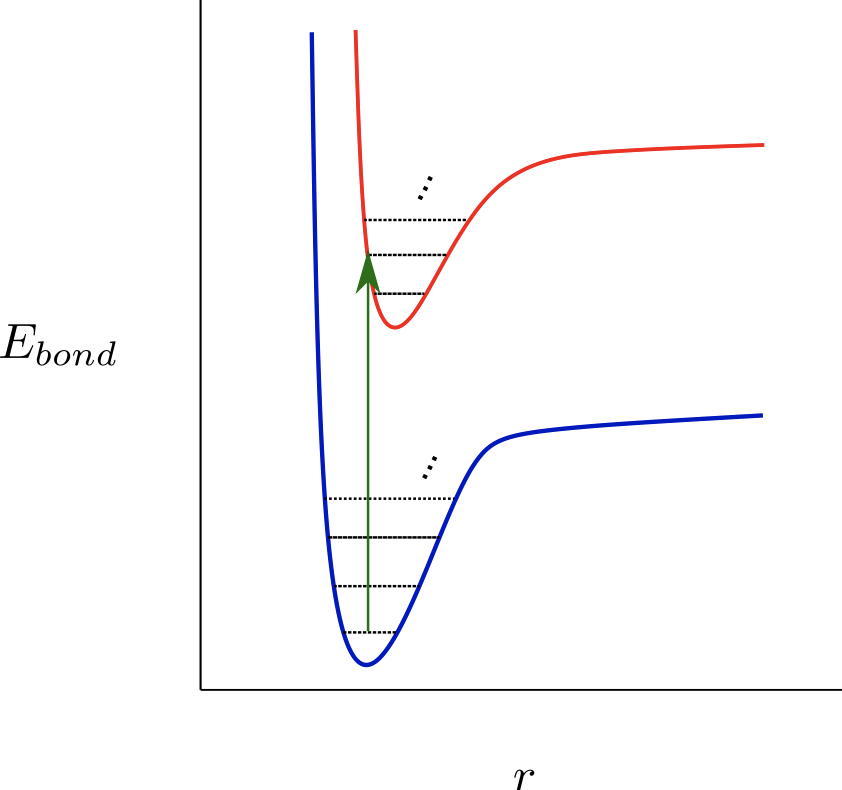
\includegraphics[width=0.4\linewidth]{figures/potential_energy_curve.pdf}
    \end{center}
    \caption{
        The general form of a molecule's potential energy curve as a function of bond length. The blue curve represents a molecule in its ground electronic state and the red curve represents the same molecule in an excited electronic state.
    }
    \label{fig:potential_curve}
\end{figure}

Vibrations affect the distance between the atoms, $r$, in the molecule. It turns out that the laws of quantum mechanics only allow for \textit{discrete} vibrational energies, and that the lowest vibrational energy that can be obtained (dubbed the ``ground'' vibrational state) is actually slightly above the minimum point on the blue/red curve. The allowed vibrational energy levels of the molecule are the horizontal lines within the blue curve in Fig.~\ref{fig:potential_curve}.

We can also think about exciting the molecule's electrons. If we were to do this, this can drastically change the interplay between the attractive and repulsive forces. Therefore, $E_{bond}$ as a function of $r$ changes significantly. The red and blue curves in Fig.~\ref{fig:potential_curve} are meant to represent the molecule in an excited electronic state and in its ground (lowest energy) electronic state, respectively. Note that the excited electronic state of the molecule also vibrates and therefore has its own discrete vibrational energy levels.

\subsubsection{Wavefunctions}

We need knowledge of one more thing before we can accomplish our goal of calculating Franck Condon Factors: wavefunctions. The wavefunction of a system, often denoted by the Greek letter $\psi$, is essentially the key to being able to calculate anything and everything about said system. In our spectroscopy language, the wavefunction of a molecule that we are interested in can be extremely complicated to fully determine. However, for our purposes we can ``separate'' the wavefunction of our molecule into parts describing its vibration ($v$), rotation ($R$) and electrons ($e$).
\begin{equation}
    \psi_{molecule} = \psi_e\psi_R\psi_v
\end{equation}

\subsubsection{Franck Condon Factors}

Armed with this conceptual knowledge of molecular vibrational energy levels and wavefunctions, we can now learn about Franck Condon Factors (FCFs). Picture the following scenario. We have a molecule in its ground state (both vibrationally and electronically), and we excite it electronically (i.e. move from the blue curve to the red curve in Fig.~\ref{fig:potential_curve}). To a very good approximation, it turns out that electronic transitions are so fast that the distance separating atoms in a molecule does not have time to adjust (this is the Franck Condon Principle). Diagrammatically, we are looking at the vertical green line in Fig.~\ref{fig:potential_curve} (it is vertical because the atoms in the molecule stays at the same distance apart during the transition). This specific ``vertical'' transition from the ground electronic and vibrational state to the excited electronic state and its second vibrational state will have a \textit{transition intensity} that is related to the vibrational part of the wavefunctions describing the system before and after the transition. More specifically, the transition intensity is proportional to the square \textit{overlap} (think of a vector dot product) between the two vibrational wavefunctions.
\begin{equation}
    \text{Transition}\text{ intensity} \propto \text{overlap}(\psi_{v,\text{before}},\psi_{v,\text{after}})^2
\end{equation}
The square of this overlap is precisely the Franck Condon Factor!
\begin{equation} \label{eq:FCF}
    \text{FCF} = \text{overlap}(\psi_{v,\text{before}},\psi_{v,\text{after}})^2
\end{equation}

\subsubsection{A simplified model for vibrations of diatomic molecules (2-atom molecules)}

We've now developed the idea of a Franck Condon Factor (FCF). How do we formally calculate these quantities?
As evident in Eq.~\eqref{eq:FCF}, we require knowledge of the {\it vibrational wavefunction} before and after the transition.
One of the simplest ways to represent vibrations of diatomic molecules is to consider that they are connected by a spring.
This ``spring system'' is usually referred to in the scientific community as a {\it harmonic oscillator}. Let's now look into this description of molecular vibrations.

In section ~\ref{sec:molec_energy_lvls}, you learned that vibrational energy levels are discrete.
Fig.~\ref{fig:harmonic_curve} shows how the vibrational energy levels are spaced in the harmonic oscillator picture. If a molecule is in it's ground vibrational state, it will ``stretch'' and ``contract" about it’s natural (or equilibrium) bond length. As it gains energy and moves into excited vibrational states, it can stretch and contract further and further from it’s equilibrium bond length. The frequency of the vibration -- how many times in one second that the molecule's spring fully extends, then fully contracts, and comes back again -- is directly related to how strong the bond is between the atoms (i.e. how ``stiff'' the spring is).

\begin{figure}
    \begin{center}
        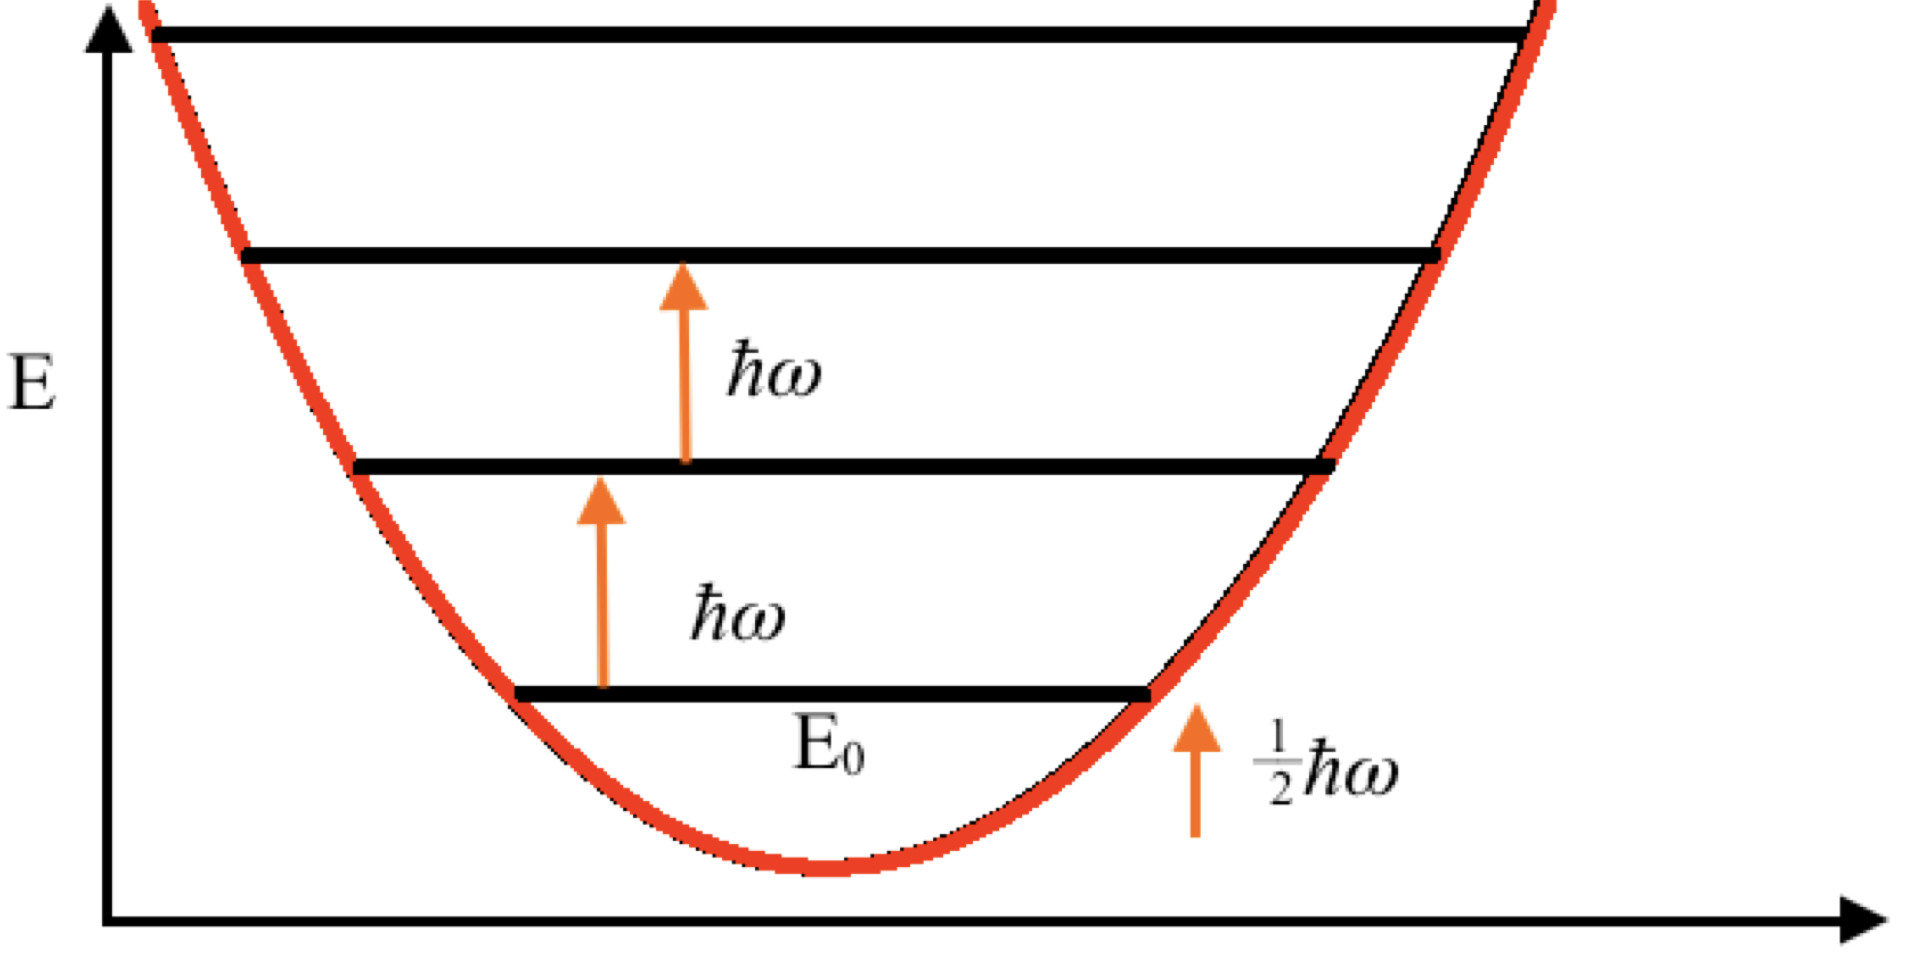
\includegraphics[width=0.4\linewidth]{figures/Harmonic_Oscillator.pdf}
    \end{center}
    \caption{
        A representation of a diatomic and it's vibrational energy levels in the harmonic oscillator approximation. The properties of this diatomic molecule are it's equilibrium geometry, $x_{eq}$, it's frequency, $\omega$, and it's reduced mass, $\mu$. The ground state energy ($E_0$) is $\frac{1}{2}\hbar\omega$ above the potential minimum and vibrational energy differences between adjacent levels is $\hbar\omega$.
    }
    \label{fig:harmonic_curve}
\end{figure}

The harmonic oscillator is an extremely simplified model, since it ignores all repulsive effects of the 2 atoms within the molecule (the steep wall at small $r$ denoted by a more realistic potential energy curve in Fig.~\ref{fig:potential_curve}). On top of this, the harmonic oscillator potential has no dissociation (or bond-breaking) as is captured by the flat portion at large $r$ in the potential energy curve in Fig.~\ref{fig:potential_curve}. In our harmonic oscillator picture, this means that at higher excited states the atoms will continue to stretch further and further without the ``spring snapping.''

However, the harmonic oscillator has a useful feature in that the energy levels are equally spaced and the vibrational wavefunction (what we need to calculate FCFs) takes a ``nice'' analytic form, allowing for simple calculations. The $n^{th}$ state of the harmonic oscillator has the following vibrational wavefunction.
\begin{equation}
    \psi_{v,n}(x) = \frac{1}{\sqrt{2^nn!}}\left(\frac{\mu\omega}{\pi\hbar}\right)\cdot\exp\left(-\frac{\mu\omega (x-x_{eq})^2}{2\hbar}\right)\cdot H_n\left(\sqrt{\frac{\mu\omega}{\hbar}}(x-x_{eq})\right) \qquad n=0,1,2,...
\end{equation}
$\mu$ is the reduced mass of the molecule, $\omega$ is it's fundamental vibrational frequency, $x$ is the bond length, $x_{eq}$ is the equilibrium bond length, $n$ is the vibrational state of the system, and $H_n$ is called a {\it Hermite polynomial}.\footnote{Check this Wikipedia article out to read more on Hermite polynomials: \href{https://en.wikipedia.org/wiki/Hermite_polynomials}{\textcolor{blue}{wikipedia.org}}.}.

With this information, we can begin actually calculating FCFs! Start with reading the documentation for Project 3.\footnote{\href{https://github.com/CDL-Quantum/CohortProject_2020/tree/master/Project_3_Franck_Condon_Factors}
    {\textcolor{blue}{https://github.com/CDL-Quantum/}}}
You will explore techniques to calculate FCFs.
Once you've mastered these techniques and have finished the tasks, you're encouraged to continue with one of the {\it Challenges} provided (or better yet, make up your own)!

\subsection{Week 4: Ising Annealer}

Numerical methods are often developed with little consideration for application in the sciences. Early Monte Carlo methods were no exception. Initially, Monte Carlo methods were designed to approximate very difficult integrals (i.e. functions that behave unidealy and very high dimensional integrals). We encourage you to visit the Wikipedia article\footnote{\href{http://en.wikipedia.org/wiki/Monte\_Carlo\_integration}{wikipedia.org/wiki/Monte\_Carlo\_integration}} on MC integration methods. There are some interesting examples to work through! For now, let's focus on how we will be employing MC methods to solve your week 4 tasks. 

\subsubsection{Monte Carlo Simulations (Metropolis-Hastings)}

In statistical physics at finite temperature, the partition function, 
\begin{equation} \label{eq:partition_fn}
    Z = \sum_{\sigma} e^{-\beta E(\sigma)},
\end{equation}
is what we wish to calculate in order to fully determine the equilibrium properties of a system of interest. Here, $\sigma$ describes one of many possible microscopic configurations that a system can be in, $E(\sigma)$ is the corresponding energy of the configuration $\sigma$, and $\beta \propto \frac{1}{T}$ where $T$ is the temperature of the system. It turns out the the probability of the system being in a configuration $\sigma$ is\footnote{We are disregarding any degeneracies here.}
\begin{equation} \label{eq:probability}
    p(\sigma) = \frac{e^{-\beta E(\sigma)}}{Z}.
\end{equation}
Our goal will be to sample configurations $\sigma$ from this probability distribution. However, this can rarely be done directly because the partition function, Eq.~\eqref{eq:partition_fn}, requires resources exponential in system size to compute. We are once again met with the {\it curse of dimensionality}!

Since we will once again be working in the language of spin-$1/2$ particles as in Projects 1 and 2, we may think of configurations $\sigma$ as being spin configurations. For a system of $N$ particles, a spin configuration is simply $N$ bits (0's and 1's). Suppose that we start with a spin configuration that may or may not be a very probable spin configuration that the system could be in. Our goal will be to modify said configuration in such a way that after several calculated modifications we will have essentially sampled the probability distribution given by Eq.~\eqref{eq:probability}. How do we modify the initial configuration and how do we know that the modification we made is a good one?

Systems lie in states that minimize their energy. Therefore, if we propose modifications to the initial configuration such that the new configuration has a lower energy, we should always accept that modification. On the flip side, if the new configuration we propose has a higher energy than the previous one we can accept it probabilistically. This is, essentially, the Metropolis-Hastings algorithm. Here it is in a little more detail. 
\begin{enumerate}
    \item Choose a random spin configuration $\sigma$ to start. 
    \item Randomly choose a spin in the configuration and flip it (i.e. $0 \rightarrow 1$ or $1 \rightarrow 0$). Call this new configuration $\sigma^{\prime}$.
    \item Accept this new configuration with probability
        \begin{equation} \label{eq:acceptance}
            P_{\text{accept}} = \text{min}\left(1, \frac{e^{-\beta E(\sigma^\prime)}}{e^{-\beta E(\sigma)}}\right)
        \end{equation}
    \item If you accepted the update, let $\sigma = \sigma^\prime$. Otherwise, discard $\sigma^\prime$. 
    \item Repeat step 2.
\end{enumerate}
The number of times that we repeat step 2 in the above list is typically called the {\it number of MC steps}.

Of course, we've intentionally kept this introduction to Monte Carlo methods very brief and we've left out many important details. However, this should be enough to get you started. If you want to learn more check out Ref.~\cite{NewmanMC}.

\subsubsection{Annealing}

MC simulations that use the single-flip MH algorithm as outlined previously work well in a lot of cases. However, sometimes these simulations fail at lower and lower temperatures. Consider for moment that we performed a MC simulation at a higher temperature $T_1$ and we've obtained good samples from the system of interest at temperature $T_1$. If we were to look at the system at a slightly lower temperature $T_1 - \varepsilon$, where $\varepsilon << 1$, we should expect that the samples we obtained from the simulation at $T_1$ would be very similarly distributed to samples obtained from a good simulation at $T_1 - \varepsilon$. So, if we use the samples from the $T_1$ simulation as our starting configurations for a simulation at $T_1 - \varepsilon$ we should have a much easier time with completing a simulation at $T_1 - \varepsilon$.

Suppose now that our end goal is to have samples from a system at a temperature $T_2$ and that performing a MC simulation directly at $T_2$ is difficult. However, a MC simulation at $T_1$ is relatively easy. A procedure to get to an efficient simulation at $T_2$ is if we do exactly what was outlined above but many, many more times until we reach $T_2$. This is called an {\it annealing procedure}. 

With this information, you can start reading the documentation for Project 4.\footnote{\href{https://github.com/CDL-Quantum/CohortProject_2020/tree/master/Project_4_Franck_Condon_Factors}
{\textcolor{blue}{https://github.com/CDL-Quantum/}}} You will get a chance to work with a MC simulation that uses the MH algorithm and execute an annealing procedure to simulate a low-temperature system. Once you've mastered the tasks, continue on with one of the Challenges provided or make up your own!

\newpage

\bibliography{refs}
\bibliographystyle{unsrt}

\end{document}
